\documentclass[a4paper,12pt]{article}

% Các gói cần thiết cho tiếng Việt và định dạng văn bản
\usepackage[utf8]{inputenc}
\usepackage[T5]{fontenc}
\usepackage[vietnamese]{babel}
\usepackage{amsmath, amssymb}
\usepackage{geometry}
\geometry{a4paper, margin=2.5cm, bottom=3cm}
\usepackage{booktabs}
\usepackage{fancyhdr}
\usepackage{enumitem}
\usepackage{needspace}
\usepackage{titlesec}
\usepackage{graphicx}
\usepackage{float}
\usepackage{listings}
\usepackage{xcolor}
\usepackage{longtable}
\usepackage{array}
\usepackage{tabularx}
\usepackage{hyperref}

% Định nghĩa màu sắc (Phong cách hiện đại)
\definecolor{codegreen}{rgb}{0,0.6,0}
\definecolor{codegray}{rgb}{0.5,0.5,0.5}
\definecolor{codepurple}{rgb}{0.58,0,0.82}
\definecolor{backcolour}{rgb}{0.95,0.95,0.92}
\definecolor{sqlblue}{rgb}{0.0, 0.0, 0.8}

% Cấu hình listings
\lstset{
    language=SQL,
    backgroundcolor=\color{backcolour},   
    commentstyle=\color{codegreen},
    keywordstyle=\color{sqlblue}\bfseries,
    numberstyle=\tiny\color{codegray},
    stringstyle=\color{codepurple},
    basicstyle=\ttfamily\small,
    breakatwhitespace=false,         
    breaklines=true,                 
    captionpos=b,                    
    keepspaces=true,                 
    numbers=left,                    
    numbersep=5pt,                  
    showspaces=false,                
    showstringspaces=false,
    showtabs=false,                  
    tabsize=2,
    frame=single,                       % Tạo khung bao quanh code
    rulecolor=\color{black!30},         % Màu của khung
    title=\lstname                      % Hiển thị tên file nếu có
}

\newcommand{\assignmentClass}{Thực tập cơ sở}

% Định dạng header/footer
\pagestyle{fancy}
\fancyhf{}
\fancyhead[L]{\small\assignmentClass}
\fancyfoot[C]{\thepage}
\renewcommand{\headrulewidth}{0.4pt}
\renewcommand{\footrulewidth}{0pt}
\setlength{\headheight}{14.5pt}

% Cấu hình khoảng cách và định dạng
\setlength{\parskip}{0.3em}
\setlength{\parindent}{0pt}

% Cấu hình danh sách
\setlist[itemize]{
    topsep=0.2em,
    itemsep=0.1em,
    partopsep=0.2em,
    parsep=0.1em,
    leftmargin=1.5em
}

% ============================================================
% PHẦN CHỈNH SỬA: XÓA SỐ SECTION, GIỮ SUBSECTION DẠNG 1., 2.
% ============================================================

% 1. Định nghĩa lại cách hiển thị số (để hiện trong mục lục)
\renewcommand{\thesection}{} % Xóa số của Section
\renewcommand{\thesubsection}{\arabic{subsection}.} % Subsection dạng 1., 2.
\renewcommand{\thesubsubsection}{\arabic{subsection}.\arabic{subsubsection}}

% 2. Định dạng lại font và khoảng cách cho tiêu đề
\titleformat{\section}
  {\normalfont\Large\bfseries}
  {} % Không có nhãn (label) cho section
  {0pt} % Khoảng cách thụt đầu dòng bằng 0
  {}

\titleformat{\subsection}
  {\normalfont\large\bfseries}
  {\thesubsection} % Hiển thị số 1., 2.
  {0.5em} % Khoảng cách giữa số và chữ
  {}

% Giữ nguyên titlespacing cũ của bạn
\titlespacing*{\section}{0pt}{0.8em}{0.4em}
\titlespacing*{\subsection}{0pt}{0.6em}{0.3em}
\titlespacing*{\subsubsection}{0pt}{0.4em}{0.2em}

% Reset số của subsection mỗi khi sang Section mới (nếu muốn bắt đầu lại từ 1)
\makeatletter
\@addtoreset{subsection}{section}
\makeatother
% ============================================================

\begin{document}
% Tiêu đề
\newcommand{\thisfancypage}[1]{%
  \setlength{\fboxsep}{0pt}
  \fbox{#1}%
}

\begin{center}
    {\fontsize{13pt}{1}\selectfont\textbf{HỌC VIỆN CÔNG NGHỆ BƯU CHÍNH VIỄN THÔNG}}\\
    {\fontsize{13pt}{1}\selectfont\textbf{KHOA CÔNG NGHỆ THÔNG TIN}}\\[0.5cm]
    \rule{10cm}{0.4pt}\\[0.2cm]
    \textbf{--------------------  o0o  --------------------}\\[1cm]

    
\includegraphics[scale=0.2]{images/logoTruong.png} \\[1.5cm] % Bỏ comment nếu bạn đã có file ảnh

    {\fontsize{15pt}{1}\selectfont\textbf{BÁO CÁO}}\\
    {\fontsize{15pt}{1}\selectfont\textbf{MÔN: THỰC TẬP CƠ SỞ}}\\[0.5cm]

    {\fontsize{15pt}{1}\selectfont\textbf{NHÓM 5}}\\[0.25cm]
    {\fontsize{18pt}{1}\selectfont\textbf{ĐỀ TÀI: XÂY DỰNG HỆ THỐNG BLOG CÁ NHÂN}}\\
\end{center}

\begin{flushleft}
\hspace{2.6 cm} \begin{tabular}{l @{\hspace{1.5cm}} l}
    \textbf{\large Hoàng Văn Chính} & \textbf{\large B23DCKH011} \\[0.2cm]
\end{tabular}
\end{flushleft}

\begin{center}
\vfill
\textbf{{\large Hà Nội - 2026}}\\
\end{center}
\vspace{1em}
\newpage
\tableofcontents
\newpage

\begin{center}
    \textbf{\LARGE Xây dựng hệ thống Blog cá nhân}
\end{center}
\vspace{1em}

\section{CHƯƠNG 1: GIỚI THIỆU ĐỀ TÀI}

\subsection{Đặt vấn đề}
Trong bối cảnh công nghệ thông tin phát triển và thay đổi liên tục, việc cập nhật kiến thức mới là một yêu cầu bắt buộc đối với mỗi lập trình viên cũng như những người làm việc trong lĩnh vực kỹ thuật. Quá trình tiếp thu các ngôn ngữ, framework hay những nguyên lý thiết kế phần mềm thường diễn ra với tốc độ rất nhanh. Tuy nhiên, hệ quả của việc "học nhanh" là bộ não con người khó có thể ghi nhớ toàn bộ và tường tận mọi chi tiết kỹ thuật trong thời gian dài.

Do đó, thói quen vừa học vừa ghi chép, hệ thống hóa lại tài liệu là một giải pháp thiết yếu. Việc lưu trữ lại những bài học chuyên môn (ví dụ như các khái niệm về lập trình hướng đối tượng, cách triển khai một kiến trúc phần mềm, hay các thủ thuật tối ưu hóa cơ sở dữ liệu) không chỉ giúp củng cố kiến thức tại thời điểm học mà còn tạo ra một "bộ nhớ ngoài" đắc lực để dễ dàng tra cứu lại khi cần thiết trong công việc thực tế.

Hơn thế nữa, tri thức sẽ sinh sôi khi được chia sẻ. Nhu cầu công khai các bài viết, bài nghiên cứu cá nhân để giao lưu, trao đổi với cộng đồng cũng ngày một tăng cao. Xuất phát từ những nhu cầu thực tiễn đó, đề tài \textbf{"Xây dựng hệ thống Blog cá nhân"} được lựa chọn nghiên cứu và phát triển. Ứng dụng này sẽ cung cấp một không gian riêng tư và chuyên nghiệp để tác giả biên soạn bài viết bằng Markdown, đồng thời là nơi lưu trữ, phân loại theo các chủ đề (topics) và chuỗi bài học (series) đồng thời chia sẻ kiến thức đến với mọi người.

\subsection{Mục tiêu đề tài}
Đề tài hướng tới việc xây dựng một hệ thống website blog cá nhân hoàn chỉnh với các mục tiêu cụ thể sau:

\begin{itemize}
    \item \textbf{Về mặt tiện ích:} Tạo ra một nền tảng cho phép người quản trị (admin) dễ dàng đăng tải, quản lý các bài viết học thuật được soạn thảo dưới định dạng Markdown (định dạng tối ưu nhất cho dân kỹ thuật). Ngoài ra quản lý các chủ đề (Topics) và chuỗi bài học (Series) của bài viết.
    \item \textbf{Về mặt trải nghiệm:} Cung cấp giao diện trực quan, dễ sử dụng cho người đọc (khách) khi truy cập để tìm kiếm, theo dõi các bài viết theo từng chuyên mục hoặc theo các chuỗi bài viết (series) liên quan với nhau.
    \item \textbf{Về mặt kỹ thuật:} Vận dụng và kết hợp thành thạo các kiến thức đã học về phát triển ứng dụng Web, bao gồm việc xây dựng giao diện phía người dùng (Frontend), thiết kế API và xử lý logic nghiệp vụ phía máy chủ (Backend), cũng như quản trị cơ sở dữ liệu.
\end{itemize}

\subsection{Phạm vi đề tài}
Do giới hạn về thời gian của môn học thực tập cơ sở, hệ thống sẽ tập trung vào các chức năng cốt lõi nhất của một blog cá nhân, bao gồm:

\begin{itemize}
    \item \textbf{Đối với khách (Guest):} Truy cập trang chủ; xem danh sách bài viết mới nhất; phân loại bài viết theo các chủ đề (Topics) và chuỗi bài học (Series). Đọc chi tiết bài viết với giao diện hiển thị rõ ràng. Xem thông tin, phương thức liên hệ của chủ website.
    \item \textbf{Đối với quản trị viên (Admin):} Có cơ chế đăng nhập bảo mật. Quản lý (Thêm, sửa, xóa, ẩn/hiện) các bài viết, danh mục và series. Trực tiếp soạn thảo bài viết bằng công cụ hỗ trợ Markdown. Cập nhập thông tin và phương thức liên hệ của bản thân.
\end{itemize}

\subsection{Công nghệ sử dụng}
Để đáp ứng các yêu cầu về hiệu năng, tính mở rộng và trải nghiệm người dùng, hệ thống được xây dựng dựa trên các công nghệ sau:

\begin{itemize}
    \item \textbf{Frontend (Giao diện người dùng):} Sử dụng \textbf{ReactJS}. Đây là một thư viện JavaScript phổ biến giúp xây dựng giao diện người dùng theo dạng các component độc lập, mang lại trải nghiệm mượt mà, tốc độ phản hồi nhanh (Single Page Application) và rất phù hợp để xử lý giao diện hiển thị Markdown động.
    \item \textbf{Backend (Xử lý nghiệp vụ):} Sử dụng \textbf{Java Spring Boot}. Nền tảng này cung cấp cấu trúc kiến trúc vững chắc, bảo mật cao và tối ưu cho việc xây dựng các RESTful API phục vụ cho quá trình giao tiếp dữ liệu với Frontend.
    \item \textbf{Hệ quản trị Cơ sở dữ liệu:} Sử dụng \textbf{MySQL}. Là một hệ quản trị cơ sở dữ liệu quan hệ mạnh mẽ, lưu trữ và truy xuất các dữ liệu có cấu trúc một cách an toàn và hiệu quả (bao gồm thông tin người dùng, bài viết, chuyên mục).
\end{itemize}

\vspace{1em}
\hrule
\vspace{1em}

\section{CHƯƠNG 2: TÀI LIỆU PHA YÊU CẦU CỦA HỆ THỐNG}

\subsection{Bảng thuật ngữ}

\begin{longtable}{|p{3.5cm}|p{3.5cm}|p{8cm}|}
\hline
\textbf{Thuật ngữ (Tiếng Anh)} & \textbf{Thuật ngữ (Tiếng Việt)} & \textbf{Ý nghĩa} \\
\hline
\textbf{Markdown} \textit{(n)} & Ngôn ngữ đánh dấu & Là một ngôn ngữ đánh dấu văn bản nhẹ, cho phép người viết sử dụng các ký tự thông thường để định dạng văn bản (in đậm, in nghiêng, chèn khối mã nguồn). Hệ thống sẽ tự động render thành HTML trực quan. \\
\hline
\textbf{Topics} \textit{(n)} & Các chủ đề & Là nhóm phân loại bài viết theo một chủ đề, lĩnh vực kỹ thuật hoặc ngôn ngữ lập trình cụ thể (Ví dụ: Lập trình Web, Database, Java Core). \\
\hline
\textbf{Series} \textit{(n)} & Chuỗi bài & Là tập hợp các bài viết có tính tuần tự, liên kết chặt chẽ với nhau để tạo thành một lộ trình hướng dẫn chi tiết từ cơ bản đến nâng cao. \\
\hline
\textbf{Post} \textit{(n)} & Bài viết & Đơn vị nội dung cơ bản của blog, chứa kiến thức, chia sẻ hoặc tài liệu học thuật do tác giả biên soạn. \\
\hline
\textbf{Trending} \textit{(adj)} & Thịnh hành / Nổi bật & Trạng thái của các bài viết nhận được nhiều sự quan tâm, lượt xem lớn hoặc được đánh giá cao trong một khoảng thời gian nhất định. \\
\hline
\textbf{Profile} \textit{(n)} & Hồ sơ cá nhân & Khu vực lưu trữ thông tin giới thiệu về tác giả và các phương thức liên hệ (Email, GitHub, LinkedIn,...). \\
\hline
\textbf{Admin} \textit{(n)} & Quản trị viên & Là chủ sở hữu của website, người có toàn quyền đăng nhập để quản lý nội dung, danh mục, chuỗi bài và thông tin cá nhân. \\
\hline
\textbf{Guest / Reader} \textit{(n)} & Khách vãng lai & Là những người truy cập vào hệ thống website để đọc tài liệu, tìm kiếm kiến thức mà không cần tài khoản đăng nhập. \\
\hline
\end{longtable}

\subsection{Mô hình nghiệp vụ bằng ngôn ngữ tự nhiên}

\textbf{2.1. Mục tiêu và phạm vi hệ thống}
\begin{itemize}
    \item \textbf{Mục tiêu:} Xây dựng một website cá nhân để lưu trữ, hệ thống hóa và chia sẻ kiến thức chuyên môn. Hệ thống tối ưu hóa trải nghiệm soạn thảo mã nguồn bằng Markdown và tạo kênh kết nối giữa tác giả với cộng đồng lập trình viên thông qua phần thông tin liên hệ.
    \item \textbf{Phạm vi:} Trọng tâm của phần mềm là hệ thống quản trị nội dung (CMS) cơ bản tập trung vào Bài viết, Chuyên mục, Series; xử lý hiển thị bài viết mới và trang thông tin liên hệ cá nhân.
\end{itemize}

\textbf{2.2. Ai có thể sử dụng phần mềm?}

Hệ thống phục vụ hai nhóm đối tượng chính:
\begin{enumerate}
    \item \textbf{Quản trị viên (Admin):} Tác giả của blog.
    \item \textbf{Khách (Guest):} Bất kỳ ai truy cập vào blog thông qua mạng Internet.
\end{enumerate}

\textbf{2.3. Người dùng có những chức năng gì?}
\begin{itemize}
    \item \textbf{Với Admin:} Đăng nhập hệ thống; Quản lý (Thêm, sửa, xóa) Topics và Series; Soạn thảo, xuất bản và quản lý Bài viết; Cập nhật thông tin giới thiệu và phương thức liên hệ của bản thân.
    \item \textbf{Với Guest:} Xem trang chủ với danh sách bài viết mới nhất; Xem danh sách bài theo Chuyên mục/Series; Đọc chi tiết bài viết (giao diện Markdown render); Xem thông tin tác giả và phương thức liên hệ.
\end{itemize}

\textbf{2.4. Mỗi chức năng hoạt động ra sao?}
\begin{itemize}
    \item \textbf{Luồng hoạt động của Guest:} Khi truy cập, Guest sẽ thấy Trang chủ hiển thị nổi bật các bài viết mới cập nhật và thông tin của tác giả. Guest có thể duyệt qua thanh menu để lọc bài viết theo Topic hoặc Series, tìm kiếm bài viết. Khi nhấn vào bài viết, nội dung Markdown sẽ được hiển thị rõ ràng với các khối mã (code block) dễ đọc.
    \item \textbf{Luồng hoạt động của Admin:} Admin truy cập trang đăng nhập ẩn và xác thực. Tại Dashboard, Admin có thể cập nhật hồ sơ cá nhân của mình. Khi học được kiến thức mới, Admin tạo Bài viết, gõ nội dung bằng Markdown, chọn trạng thái (Lưu nháp hoặc Xuất bản) và gắn vào Topic/Series tương ứng. Các thay đổi này sẽ lập tức phản ánh lên giao diện của Guest sau khi lưu.
\end{itemize}

\textbf{2.5. Những thông tin/ đối tượng mà hệ thống cần xử lý}

Hệ thống thao tác với 4 thực thể dữ liệu chính:
\begin{enumerate}
    \item \textbf{Thông tin tác giả (Profile/Users):} Tài khoản đăng nhập, Mật khẩu (mã hóa), Họ tên, Ảnh đại diện, Giới thiệu ngắn, Link liên hệ (Github, Facebook, LinkedIn).
    \item \textbf{Bài viết (Posts):} Tiêu đề, Chuỗi URL (Slug), Nội dung Markdown, Ngày tạo, Lượt xem (để tính trending), Trạng thái (Draft/Published).
    \item \textbf{Chủ đề (Topics):} Tên chủ đề, Mô tả.
    \item \textbf{Chuỗi bài (Series):} Tên chuỗi, Mô tả lộ trình.
\end{enumerate}

\textbf{2.6. Quan hệ giữa các đối tượng}
\begin{itemize}
    \item Một \textbf{Chủ đề} chứa \textit{nhiều} \textbf{Bài viết}. Một \textbf{Bài viết} cũng có thể thuộc \textit{nhiều} \textbf{Chủ đề}.
    \item Một \textbf{Series} chứa \textit{nhiều} \textbf{Bài viết}. Một \textbf{Bài viết} có thể thuộc hoặc \textit{không thuộc} \textbf{Series} nào.
\end{itemize}

\subsection{Mô hình nghiệp vụ bằng UML}

\textbf{3.1. Xác định các actor của hệ thống}
\begin{itemize}
    \item \textbf{Guest (Khách):} Tác nhân đại diện cho người đọc (không cần xác thực).
    \item \textbf{Admin (Quản trị viên):} Tác nhân đại diện cho chủ sở hữu hệ thống. (Admin sẽ kế thừa mọi quyền hạn của Guest).
\end{itemize}

\textbf{3.2. Các use case cho từng actor}
\begin{itemize}
    \item \textbf{Actor: Guest}
    \item \texttt{UC01: Truy cập trang chủ (danh sách bài viết, thông tin tác giả)}
    \item \texttt{UC02: Lọc bài viết theo Topic / Series}
    \item \texttt{UC03: Tìm kiếm bài viết}
    \item \texttt{UC04: Xem chi tiết bài viết}
\end{itemize}

\begin{itemize}
    \item \textbf{Actor: Admin}
    \item \texttt{UC05: Đăng nhập hệ thống}
    \item \texttt{UC06: Quản lý Chuyên mục (Thêm, sửa, xóa)}
    \item \texttt{UC07: Quản lý Series (Thêm, sửa, xóa)}
    \item \texttt{UC08: Quản lý bài viết (Xem danh sách bài viết, xóa bài viết)}
    \item \texttt{UC09: Thêm bài viết mới}
    \item \texttt{UC10: Chỉnh sửa bài viết}
    \item \texttt{UC11: Cập nhật thông tin cá nhân và phương thức liên hệ}
    \item \texttt{UC12: Đăng xuất}
\end{itemize}

\begin{figure}[H]
    \centering
    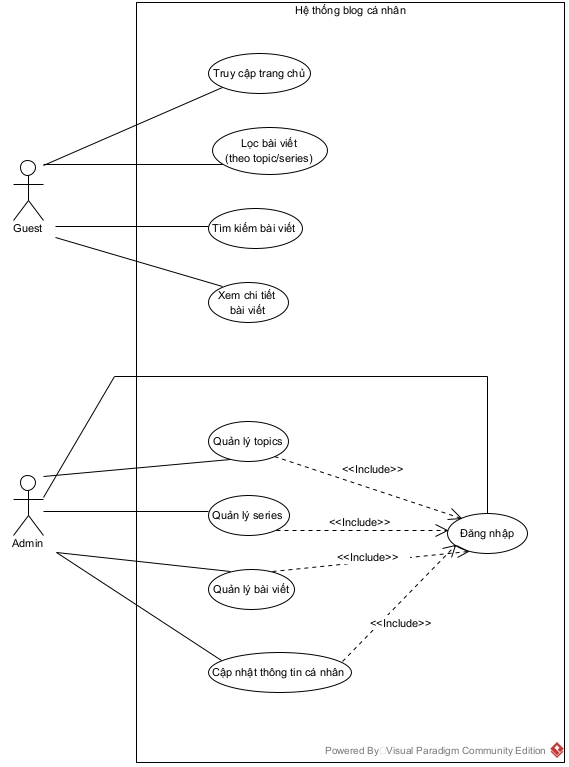
\includegraphics[height=1.0\textwidth]{use_case_diagram/Blog_UCD.jpg}

    \caption{Biểu đồ Use Case tổng quát}
\end{figure}

\subsection{Bảng yêu cầu người dùng}

\begin{longtable}{|c|p{10.5cm}|c|}
\hline
\textbf{ID} & \textbf{Mô tả yêu cầu} & \textbf{Độ ưu tiên} \\
\hline
\textbf{FR01} & Khách truy cập có thể xem danh sách bài viết mới nhất và tìm kiếm bài viết trên trang chủ. & Cao \\
\hline
\textbf{FR02} & Khách truy cập có thể lọc và tìm kiếm các bài viết theo từng Topic hoặc Series cấu trúc sẵn. & Cao \\
\hline
\textbf{FR03} & Khách truy cập có thể đọc chi tiết bài viết với giao diện Markdown đã được render hoàn chỉnh (hiển thị rõ cấu trúc text, code block, hình ảnh). & Cao \\
\hline
\textbf{FR04} & Khách truy cập có thể xem thông tin giới thiệu về tác giả và các phương thức liên hệ (Facebook, Github, LinkedIn) trên trang chủ & Trung bình \\
\hline
\textbf{FR05} & Hệ thống cung cấp cơ chế đăng nhập bảo mật dành riêng cho Quản trị viên (Admin). & Cao \\
\hline
\textbf{FR06} & Quản trị viên có trình soạn thảo văn bản hỗ trợ cú pháp Markdown để tạo mới, chỉnh sửa bài viết. & Cao \\
\hline
\textbf{FR07} & Quản trị viên có thể thiết lập trạng thái bài viết: Lưu nháp (Draft) hoặc Xuất bản (Published). & Cao \\
\hline
\textbf{FR08} & Quản trị viên có thể gắn bài viết vào một Chuyên mục và/hoặc một Series cụ thể khi đăng bài. & Cao \\
\hline
\textbf{FR09} & Quản trị viên có quyền thêm mới, cập nhật tên/mô tả hoặc xóa các Chuyên mục và Series. & Cao \\
\hline
\textbf{FR10} & Quản trị viên có thể chỉnh sửa, cập nhật thông tin tiểu sử cá nhân và các đường dẫn liên hệ của mình trên hệ thống. & Trung bình \\
\hline
\end{longtable}

\section{CHƯƠNG 3: TÀI LIỆU PHA PHÂN TÍCH CỦA HỆ THỐNG}

\subsection{Use Case Specification}

\subsubsection{UC01: Truy cập trang chủ}
\begin{longtable}{|p{4cm}|p{11.5cm}|}
\hline
\textbf{Use Case ID} & UC01 \\ \hline
\textbf{Use Case Name} & Truy cập trang chủ \\ \hline
\textbf{Description} & Là Khách truy cập (Guest), tôi muốn truy cập vào trang chủ của Blog để xem các bài viết mới nhất và thông tin, phương thức liên hệ của tác giả. \\ \hline
\textbf{Actor(s)} & Guest \\ \hline
\textbf{Trigger} & Người dùng nhập địa chỉ trang web hoặc chọn biểu tượng quay về trang chủ. \\ \hline
\textbf{Pre-Condition(s)} & Hệ thống đang trong trạng thái sẵn sàng phục vụ. \\ \hline
\textbf{Post-Condition(s)} & Giao diện trang chủ được hiển thị đầy đủ thông tin cá nhân của tác giả và danh sách các bài viết đã xuất bản. \\ \hline
\textbf{Basic Flow} & 
1. Người dùng gửi yêu cầu truy cập trang chủ của hệ thống. \newline
2. Hệ thống truy xuất dữ liệu hồ sơ (Profile) của tác giả, bao gồm: Họ tên, Ảnh đại diện, Giới thiệu ngắn và Các liên kết mạng xã hội. \newline
3. Hệ thống tiếp tục truy xuất danh sách các bài viết (được sắp xếp theo ngày tạo giảm dần) và đáp ứng điều kiện hiển thị (BR01.1). \newline
4. Hệ thống tổng hợp dữ liệu và hiển thị giao diện Trang chủ cho người dùng, bao gồm khu vực giới thiệu tác giả và danh sách bài viết. \newline
5. Người dùng xem thông tin và danh sách bài viết trên trang chủ. \\ \hline
\textbf{Alternative Flow} & 
3a. Hệ thống nhận thấy hiện tại không có bài viết nào thỏa mãn điều kiện hiển thị (Blog mới tạo hoặc chưa có bài viết được xuất bản). \newline
3a1. Hệ thống trả về danh sách bài viết rỗng. \newline
3a2. Hệ thống chủ động hiển thị giao diện thông báo thay thế tại khu vực bài viết: "Hiện tại tác giả chưa xuất bản bài viết nào. Bạn vui lòng quay lại sau nhé!". \newline
Use Case kết thúc. \\ \hline
\textbf{Exception Flow} & 
Không có \\ \hline
\textbf{Business Rules} & 
BR01.1: Trạng thái hiển thị: Chỉ những bài viết có trạng thái là \texttt{Published} (Xuất bản) mới được phép lấy ra từ cơ sở dữ liệu để hiển thị cho người dùng. Bỏ qua tất cả các bài viết \texttt{Draft} (Lưu nháp). \\ \hline
\textbf{Non-Functional Requirement} & 
NFR01.1: Hiệu năng tải trang: Hệ thống phải phản hồi và hiển thị đầy đủ nội dung trang chủ trong thời gian tối đa 2 giây kể từ khi nhận được yêu cầu. \newline
NFR01.2: Tương thích hiển thị: Giao diện Trang chủ phải có khả năng tự động co giãn và hiển thị mượt mà trên nhiều kích thước màn hình thiết bị khác nhau (Máy tính, Máy tính bảng, Điện thoại di động). \\ \hline
\end{longtable}

\subsubsection{UC02: Lọc bài viết theo Topic / Series}
\begin{longtable}{|p{4cm}|p{11.5cm}|}
\hline
\textbf{Use Case ID} & UC02 \\ \hline
\textbf{Use Case Name} & Lọc bài viết theo Topic / Series \\ \hline
\textbf{Description} & Là Khách truy cập (Guest), tôi muốn lọc và xem danh sách các bài viết thuộc một Chủ đề (Topic) hoặc Chuỗi bài (Series) cụ thể để dễ dàng theo dõi các kiến thức có liên quan với nhau. \\ \hline
\textbf{Actor(s)} & Guest \\ \hline
\textbf{Trigger} & Người dùng nhấp chọn vào một Topic hoặc Series trên giao diện (từ thanh menu, danh mục hiển thị, hoặc từ nhãn gắn trên một bài viết). \\ \hline
\textbf{Pre-Condition(s)} & Hệ thống đang hoạt động ổn định và có hiển thị danh sách các Topic/Series để người dùng tương tác. \\ \hline
\textbf{Post-Condition(s)} & Giao diện hiển thị danh sách các bài viết thuộc Topic hoặc Series mà người dùng đã chọn. \\ \hline
\textbf{Basic Flow} & 
1. Người dùng thao tác nhấp chọn một Topic hoặc Series trên giao diện hệ thống. \newline
2. Hệ thống tiếp nhận yêu cầu và xác định định danh của Topic/Series được chọn. \newline
3. Hệ thống truy xuất dữ liệu chi tiết của Topic/Series đó (Tên, Mô tả ngắn). \newline
4. Hệ thống tiếp tục truy xuất danh sách các bài viết có liên kết với Topic/Series này, thỏa mãn điều kiện hiển thị (BR02.1) và sắp xếp theo quy tắc ưu tiên (BR02.2). \newline
5. Hệ thống tổng hợp dữ liệu và hiển thị giao diện trang kết quả, bao gồm: Tiêu đề, mô tả của Topic/Series và danh sách bài viết lọc được. \newline
6. Người dùng xem danh sách bài viết đã được lọc. \\ \hline
\textbf{Alternative Flow} & 
4a. Hệ thống nhận thấy Topic/Series được chọn hiện không có bài viết nào thỏa mãn điều kiện hiển thị (chưa có bài viết hoặc bài viết đang ở bản nháp). \newline
4a1. Hệ thống trả về danh sách bài viết rỗng. \newline
4a2. Hệ thống chủ động hiển thị giao diện thông báo tại khu vực danh sách: "Hiện tại chưa có bài viết nào trong chuyên mục/chuỗi bài này. Vui lòng quay lại sau!". \newline
Use Case kết thúc. \\ \hline
\textbf{Exception Flow} & 
3a. Hệ thống không tìm thấy Topic hoặc Series tương ứng trong cơ sở dữ liệu (do đã bị quản trị viên xóa hoặc đường dẫn URL không hợp lệ). \newline
3a1. Hệ thống ngừng xử lý luồng hiện tại và điều hướng người dùng sang trang thông báo lỗi 404 (Không tìm thấy nội dung). \newline
Use Case kết thúc. \\ \hline
\textbf{Business Rules} & 
BR02.1: Trạng thái hiển thị: Chỉ những bài viết có trạng thái là \texttt{Published} (Xuất bản) mới được phép lấy ra để hiển thị. \newline
BR02.2: Quy tắc sắp xếp: \newline
- Nếu lọc theo Topic: Các bài viết được sắp xếp theo ngày tạo giảm dần (bài mới nhất xếp đầu tiên). \newline
- Nếu lọc theo Series: Các bài viết bắt buộc phải được sắp xếp theo thứ tự tuần tự của chuỗi bài học (từ bài 1, bài 2,... đến bài cuối cùng) do Admin thiết lập. \newline
BR02.3: Giới hạn hiển thị (Pagination): Quy định mỗi trang chỉ hiển thị tối đa 10 bài viết. Hệ thống áp dụng cơ chế phân trang đối với các kết quả vượt quá giới hạn này. \\ \hline
\textbf{Non-Functional Requirement} & 
NFR02.1: Hiệu năng truy xuất: Hệ thống phải hoàn tất quá trình tìm kiếm, lọc và hiển thị kết quả trong thời gian tối đa 2 giây. \newline
NFR02.2: Trải nghiệm UI/UX: Giao diện trang danh mục phải cung cấp dấu hiệu nhận biết rõ ràng để người dùng biết họ đang xem nội dung thuộc Topic hay Series nào (Ví dụ: in đậm tên Topic trên tiêu đề trang). \\ \hline
\end{longtable}

\subsubsection{UC03: Tìm kiếm bài viết}
\begin{longtable}{|p{4cm}|p{11.5cm}|}
\hline
\textbf{Use Case ID} & UC03 \\ \hline
\textbf{Use Case Name} & Tìm kiếm bài viết \\ \hline
\textbf{Description} & Là Khách truy cập (Guest), tôi muốn tìm kiếm bài viết thông qua tiêu đề để nhanh chóng xác định và đọc được nội dung mà tôi đang quan tâm. \\ \hline
\textbf{Actor(s)} & Guest \\ \hline
\textbf{Trigger} & Người dùng nhập từ khóa vào ô tìm kiếm và thực hiện lệnh tìm kiếm. \\ \hline
\textbf{Pre-Condition(s)} & Hệ thống đang hoạt động và giao diện có hiển thị thanh công cụ tìm kiếm. \\ \hline
\textbf{Post-Condition(s)} & Giao diện hiển thị trang kết quả với danh sách các bài viết có tiêu đề khớp với từ khóa tìm kiếm. \\ \hline
\textbf{Basic Flow} & 
1. Người dùng nhập từ khóa tìm kiếm vào ô nhập liệu và gửi yêu cầu. \newline
2. Hệ thống tiếp nhận từ khóa và thực hiện tiền xử lý (loại bỏ các khoảng trắng thừa ở đầu và cuối từ khóa). \newline
3. Hệ thống tiến hành truy xuất danh sách các bài viết thỏa mãn đồng thời các điều kiện: tiêu đề có chứa từ khóa (BR03.2) và trạng thái hiển thị hợp lệ (BR03.1). \newline
4. Hệ thống sắp xếp các kết quả tìm được theo thời gian (ưu tiên bài viết mới nhất) và áp dụng cơ chế phân trang (BR03.3). \newline
5. Hệ thống hiển thị trang kết quả bao gồm: Dòng thông báo số lượng kết quả tìm được cho từ khóa và danh sách các bài viết. \newline
6. Người dùng xem các bài viết trên trang kết quả tìm kiếm. \\ \hline
\textbf{Alternative Flow} & 
3a. Hệ thống nhận thấy không có bài viết nào trong cơ sở dữ liệu có tiêu đề khớp với từ khóa. \newline
3a1. Hệ thống trả về danh sách kết quả rỗng. \newline
3a2. Hệ thống chủ động hiển thị giao diện thông báo tại trang kết quả: "Không tìm thấy bài viết nào phù hợp với từ khóa '[từ khóa của người dùng]'.". \newline
Use Case kết thúc. \\ \hline
\textbf{Exception Flow} & 
2a. Hệ thống phát hiện từ khóa người dùng gửi lên bị rỗng hoặc chỉ chứa các ký tự đặc biệt không hợp lệ. \newline
2a1. Hệ thống chặn yêu cầu tìm kiếm, giữ nguyên giao diện hiện tại và hiển thị cảnh báo (tooltip/toast): "Vui lòng nhập từ khóa hợp lệ để tìm kiếm". \newline
Hệ thống quay lại Bước 1. \\ \hline
\textbf{Business Rules} & 
BR03.1: Phạm vi và trạng thái tìm kiếm: Hệ thống chỉ quét từ khóa trên trường dữ liệu "Tiêu đề" của bài viết. Đồng thời, chỉ các bài viết có trạng thái \texttt{Published} (Xuất bản) mới được đưa vào tập kết quả. \newline
BR03.2: Quy tắc khớp từ: Hệ thống áp dụng tìm kiếm tương đối (chứa từ khóa) và không phân biệt chữ hoa, chữ thường (Case-insensitive). Ví dụ: Tìm "java" sẽ ra cả bài viết có tiêu đề chứa "Java" hoặc "JAVA". \newline
BR03.3: Phân trang (Pagination): Quy định mỗi trang kết quả tìm kiếm hiển thị tối đa 10 bài viết. \\ \hline
\textbf{Non-Functional Requirement} & 
NFR03.1: Hiệu năng tìm kiếm: Phản hồi kết quả tìm kiếm phải được hoàn tất và hiển thị trong thời gian tối đa 2 giây. \newline
NFR03.2: Tính khả dụng: Nếu từ khóa quá dài, hệ thống phải cắt ngắn từ khóa (hiển thị dấu ...) trên dòng thông báo kết quả để tránh vỡ giao diện. \\ \hline
\end{longtable}

\subsubsection{UC04: Xem chi tiết bài viết}
\begin{longtable}{|p{4cm}|p{11.5cm}|}
\hline
\textbf{Use Case ID} & UC04 \\ \hline
\textbf{Use Case Name} & Xem chi tiết bài viết \\ \hline
\textbf{Description} & Là Khách truy cập (Guest), tôi muốn xem toàn bộ nội dung chi tiết của một bài viết, bao gồm mục lục và các bài viết cùng chuỗi (nếu có), để tiếp thu kiến thức một cách trọn vẹn và logic. \\ \hline
\textbf{Actor(s)} & Guest \\ \hline
\textbf{Trigger} & Người dùng nhấp chọn vào tiêu đề, ảnh bìa hoặc nút "Xem chi tiết" của một bài viết. \\ \hline
\textbf{Pre-Condition(s)} & Hệ thống đang hoạt động và bài viết mục tiêu đang ở trạng thái cho phép hiển thị. \\ \hline
\textbf{Post-Condition(s)} & Giao diện hiển thị đầy đủ nội dung bài viết đã được định dạng, kèm theo mục lục và danh sách các bài viết trong cùng Series (nếu có). \\ \hline
\textbf{Basic Flow} & 
1. Người dùng yêu cầu xem chi tiết một bài viết thông qua giao diện. \newline
2. Hệ thống tiếp nhận yêu cầu và xác định định danh của bài viết. \newline
3. Hệ thống truy xuất dữ liệu chi tiết của bài viết từ cơ sở dữ liệu (Tiêu đề, Nội dung, Ngày đăng, Thông tin tác giả, Topic, Series liên kết). \newline
4. Hệ thống kiểm tra trạng thái của bài viết có thỏa mãn điều kiện hiển thị (BR04.1). \newline
5. Hệ thống phân tích nội dung bài viết, tự động trích xuất các tiêu đề mục con (Heading) để tạo thành Mục lục (Table of Contents). \newline
6. Hệ thống kiểm tra dữ liệu và nhận thấy bài viết có thuộc về một Series cụ thể. Hệ thống tiếp tục truy xuất danh sách các bài viết khác trong cùng Series này và sắp xếp theo thứ tự (BR04.2). \newline
7. Hệ thống tổng hợp dữ liệu, thực hiện chuyển đổi nội dung từ định dạng gốc (Markdown) sang định dạng hiển thị trực quan (HTML) (BR04.3). \newline
8. Hệ thống hiển thị giao diện chi tiết bài viết bao gồm: Nội dung chính, Mục lục, và Danh sách các bài cùng Series. \newline
9. Người dùng xem nội dung, tương tác với mục lục để di chuyển nhanh tới các phần, hoặc chọn đọc các bài viết khác trong cùng Series. \\ \hline
\textbf{Alternative Flow} & 
5a. Hệ thống phân tích và nhận thấy nội dung bài viết không chứa bất kỳ tiêu đề mục con (Heading) nào. \newline
5a1. Hệ thống bỏ qua quá trình tạo Mục lục và tự động ẩn khu vực hiển thị Mục lục trên giao diện chi tiết. \newline
Luồng tiếp tục tại Bước 6. \newline
6a. Hệ thống kiểm tra và nhận thấy bài viết hoạt động độc lập, không thuộc bất kỳ Series nào. \newline
6a1. Hệ thống bỏ qua việc truy xuất danh sách Series và tự động ẩn khu vực hiển thị Series trên giao diện chi tiết. \newline
Luồng tiếp tục tại Bước 7. \\ \hline
\textbf{Exception Flow} & 
3a. Hệ thống không tìm thấy bài viết trong cơ sở dữ liệu (đường dẫn URL không tồn tại hoặc bài viết đã bị xóa). \newline
3a1. Hệ thống điều hướng người dùng sang trang thông báo lỗi 404 (Không tìm thấy nội dung). \newline
Use Case kết thúc. \newline
4a. Hệ thống phát hiện bài viết có tồn tại nhưng trạng thái hiện tại không thỏa mãn điều kiện hiển thị (ví dụ: bài viết đang ở trạng thái "Draft"). \newline
4a1. Hệ thống chặn quyền truy cập nội dung và điều hướng người dùng sang trang thông báo lỗi 404 để đảm bảo bảo mật. \newline
Use Case kết thúc. \\ \hline
\textbf{Business Rules} & 
BR04.1: Trạng thái hiển thị: Chỉ những bài viết có trạng thái là \texttt{Published} (Xuất bản) mới được phép hiển thị cho Guest. Nếu bài viết là \texttt{Draft} (Lưu nháp), hệ thống coi như bài viết không tồn tại đối với quyền truy cập này. \newline
BR04.2: Hiển thị Series: Danh sách các bài viết cùng Series phải được sắp xếp theo đúng thứ tự lộ trình đã cấu hình. Bài viết người dùng đang xem hiện tại phải được làm nổi bật (highlight) trong danh sách này để định vị vị trí học tập. \newline
BR04.3: Render nội dung: Nội dung bài viết được lưu trữ dưới dạng văn bản thô có đánh dấu (Markdown) phải được hệ thống biên dịch và hiển thị chính xác các định dạng (in đậm, in nghiêng, khối mã nguồn, hình ảnh,...). \\ \hline
\textbf{Non-Functional Requirement} & 
NFR04.1: Trải nghiệm người dùng (UX): Khu vực Mục lục và Danh sách Series nên được thiết kế dưới dạng ghim cố định (sticky) bên cạnh màn hình khi người dùng cuộn nội dung bài viết để thuận tiện tra cứu. \newline
NFR04.2: Hiệu năng xử lý: Quá trình phân tích, trích xuất Heading và render nội dung phải được tối ưu hóa, đảm bảo trang chi tiết hiển thị hoàn tất trong thời gian tối đa 2 giây. \\ \hline
\end{longtable}

\subsubsection{UC05: Đăng nhập hệ thống}
\begin{longtable}{|p{4cm}|p{11.5cm}|}
\hline
\textbf{Use Case ID} & UC05 \\ \hline
\textbf{Use Case Name} & Đăng nhập hệ thống \\ \hline
\textbf{Description} & Là Quản trị viên (Admin), tôi muốn đăng nhập vào hệ thống để truy cập vào khu vực quản trị (Dashboard) và thực hiện các quyền của admin. \\ \hline
\textbf{Actor(s)} & Admin \\ \hline
\textbf{Trigger} & Admin truy cập vào đường dẫn đăng nhập dành riêng cho quản trị viên. \\ \hline
\textbf{Pre-Condition(s)} & Hệ thống đang hoạt động. Tài khoản Admin đã được khởi tạo sẵn trong cơ sở dữ liệu. Admin hiện chưa đăng nhập vào hệ thống. \\ \hline
\textbf{Post-Condition(s)} & Admin xác thực thành công, hệ thống cấp phiên làm việc hợp lệ và điều hướng Admin vào trang Quản trị (Dashboard). \\ \hline
\textbf{Basic Flow} & 
1. Admin truy cập vào trang đăng nhập của hệ thống. \newline
2. Hệ thống hiển thị biểu mẫu đăng nhập bao gồm trường Email và Mật khẩu. \newline
3. Admin nhập email và mật khẩu, sau đó nhấn xác nhận "Đăng nhập". \newline
4. Hệ thống kiểm tra dữ liệu đầu vào (kiểm tra không rỗng và đúng định dạng Email). \newline
5. Hệ thống xác thực thông tin đăng nhập khớp với dữ liệu của tài khoản Admin trong hệ thống. \newline
6. Hệ thống khởi tạo phiên làm việc bằng cách cấp phát một cặp mã xác thực (bao gồm Access Token và Refresh Token) cho Admin. \newline
7. Hệ thống điều hướng Admin tới trang Bảng điều khiển (Dashboard). \\ \hline
\textbf{Alternative Flow} & 
Không có. \\ \hline
\textbf{Exception Flow} & 
4a1. Hệ thống phát hiện trường Email hoặc Mật khẩu bị bỏ trống, hoặc trường Email nhập vào không đúng định dạng chuẩn. \newline
4a2. Hệ thống chặn yêu cầu xác thực, giữ nguyên màn hình và hiển thị cảnh báo: "Vui lòng nhập đầy đủ và đúng định dạng thông tin đăng nhập". \newline
Hệ thống quay lại Bước 3 của Basic Flow. \newline

5a1. Hệ thống phát hiện thông tin đăng nhập không chính xác. \newline
5a2. Hệ thống từ chối quyền truy cập và hiển thị thông báo lỗi chung: "Tên đăng nhập hoặc mật khẩu không chính xác" (BR05.2). \newline
Hệ thống quay lại Bước 3 của Basic Flow. \\ \hline
\textbf{Business Rules} & 
BR05.1: Tài khoản quản trị: Hệ thống Blog cá nhân là hệ thống đóng, không cung cấp tính năng Đăng ký. Chỉ có tài khoản Admin được cấu hình sẵn từ đầu (Seed data) trong cơ sở dữ liệu để sử dụng. \newline
BR05.2: Bảo mật thông báo lỗi: Khi xác thực thất bại, hệ thống tuyệt đối không thông báo chi tiết là sai "Tên đăng nhập" hay sai "Mật khẩu" để phòng tránh rủi ro kẻ gian dò quét tài khoản. \newline
BR05.3: Mã hóa mật khẩu: Quá trình đối chiếu mật khẩu tại Bước 5 phải thực hiện bằng cách so sánh chuỗi mã hóa (Hash), tuyệt đối không so sánh bằng văn bản thuần túy (Plain text). \newline
BR05.4: Cơ chế duy trì phiên (Background Refresh): Hệ thống sẽ sử dụng Refresh Token để thực hiện xác thực ngầm và tự động cấp lại Access Token mới mỗi khi thẻ cũ hết hạn, đảm bảo các thao tác của Admin trong khu vực quản trị không bị gián đoạn. \\ \hline
\textbf{Non-Functional Requirement} & 
NFR05.1: Cơ chế bảo mật Dual-Token: Phiên làm việc được quản lý thông qua hai tầng mã thông báo để tối ưu trải nghiệm và bảo mật: \newline
- Access Token (Thẻ truy cập): Thời gian sống ngắn (30 phút) nhằm giảm thiểu rủi ro nếu thẻ bị đánh cắp. \newline
- Refresh Token (Thẻ duy trì): Thời gian sống dài (30 ngày) giúp hệ thống tự động làm mới phiên, tránh việc Admin phải đăng nhập lại nhiều lần trong tháng. \newline
NFR05.2: Hiệu năng xác thực: Quá trình mã hóa, đối chiếu dữ liệu và trả về kết quả đăng nhập không được vượt quá 1.5 giây. \newline
NFR05.3: Bảo mật lưu trữ mã (Token Storage Security): Cặp mã xác thực sau khi được cấp phát cho Client bắt buộc phải được lưu trữ trong các cơ sở an toàn của trình duyệt, có thiết lập ngăn chặn triệt để sự truy cập trái phép từ các tập lệnh mã độc bên thứ ba (chống tấn công XSS). \\ \hline
\end{longtable}

\subsubsection{UC06: Quản lý Topics}
\begin{longtable}{|p{4cm}|p{11.5cm}|}
\hline
\textbf{Use Case ID} & UC06 \\ \hline
\textbf{Use Case Name} & Quản lý Topics (Chuyên mục) \\ \hline
\textbf{Description} & Là Quản trị viên (Admin), tôi muốn xem danh sách, thêm mới, chỉnh sửa hoặc xóa các Chủ đề (Topics) để phân loại và tổ chức các bài viết trên blog một cách khoa học. \\ \hline
\textbf{Actor(s)} & Admin \\ \hline
\textbf{Trigger} & Admin chọn chức năng "Quản lý Topics" trên thanh điều hướng của khu vực quản trị (Dashboard). \\ \hline
\textbf{Pre-Condition(s)} & Admin đang trong phiên đăng nhập hợp lệ. \\ \hline
\textbf{Post-Condition(s)} & Hệ thống hiển thị danh sách Topics. Mọi thay đổi về dữ liệu (thêm, sửa, xóa) được cập nhật thành công vào cơ sở dữ liệu. \\ \hline
\textbf{Basic Flow} & 
1. Admin truy cập vào chức năng Quản lý Topics. \newline
2. Hệ thống truy xuất danh sách toàn bộ các Topics hiện có từ cơ sở dữ liệu. \newline
3. Hệ thống hiển thị giao diện quản lý bao gồm danh sách Topics (Tên, Slug, Mô tả, Số lượng bài viết thuộc Topic) và các công cụ thao tác (Thêm, Sửa, Xóa). \\ \hline
\textbf{Alternative Flow} & 
3a. Thêm mới Topic: \newline
3a1. Admin chọn chức năng "Thêm mới". \newline
3a2. Hệ thống hiển thị biểu mẫu nhập liệu. \newline
3a3. Admin nhập Tên Topic, Slug, Mô tả và nhấn "Lưu". \newline
3a4. Hệ thống kiểm tra tính hợp lệ của dữ liệu (không bỏ trống, không vi phạm BR06.1). \newline
3a5. Hệ thống lưu Topic mới vào cơ sở dữ liệu, hiển thị thông báo "Thêm thành công" và cập nhật lại danh sách hiển thị. \newline
Hệ thống quay lại Bước 3 của Basic Flow. \newline

3b. Chỉnh sửa Topic: \newline
3b1. Admin chọn thao tác "Sửa" trên một Topic cụ thể trong danh sách. \newline
3b2. Hệ thống hiển thị biểu mẫu với dữ liệu hiện tại của Topic đó. \newline
3b3. Admin chỉnh sửa thông tin (Tên, Slug, Mô tả) và nhấn "Lưu". \newline
3b4. Hệ thống kiểm tra tính hợp lệ của dữ liệu (tương tự Bước 3a4). \newline
3b5. Hệ thống cập nhật thông tin vào cơ sở dữ liệu, hiển thị thông báo "Cập nhật thành công" và làm mới danh sách. \newline
Hệ thống quay lại Bước 3 của Basic Flow. \newline

3c. Xóa Topic: \newline
3c1. Admin chọn thao tác "Xóa" trên một Topic cụ thể. \newline
3c2. Hệ thống hiển thị hộp thoại cảnh báo: "Bạn có chắc chắn muốn xóa Topic này? Các bài viết thuộc Topic này sẽ bị gỡ nhãn topic". \newline
3c3. Admin xác nhận đồng ý xóa. \newline
3c4. Hệ thống tiến hành xóa Topic và xử lý gỡ liên kết các bài viết liên quan (BR06.2). \newline
3c5. Hệ thống hiển thị thông báo "Xóa thành công" và cập nhật lại danh sách. \newline
Hệ thống quay lại Bước 3 của Basic Flow. \\ \hline
\textbf{Exception Flow} & 
\textbf{E1. Lỗi xác thực dữ liệu đầu vào (Xảy ra tại Bước 3a4 hoặc Bước 3b4)} \newline
E1.1. Hệ thống phát hiện Tên Topic bị bỏ trống hoặc bị trùng lặp với một Topic đã tồn tại (Vi phạm BR06.1). \newline
E1.2. Hệ thống chặn thao tác lưu, bôi đỏ trường dữ liệu lỗi và hiển thị thông báo: "Tên Topic không hợp lệ hoặc đã tồn tại". \newline
E1.3. Hệ thống giữ nguyên biểu mẫu để Admin tiếp tục chỉnh sửa (Quay lại Bước 3a3 hoặc Bước 3b3 tùy thuộc vào luồng đang thực hiện). \\ \hline
\textbf{Business Rules} & 
BR06.1: Tính duy nhất của Topic, Slug: Tên của một Topic và Slug của nó phải là duy nhất trong toàn bộ hệ thống. \newline
BR06.2: Ràng buộc xóa (Xóa liên kết): Khi xóa một Topic, dữ liệu của các Bài viết (Posts) bên trong tuyệt đối không bị xóa. Hệ thống chỉ thực hiện thao tác gỡ bỏ liên kết giữa bài viết và Topic bị xóa. Việc một bài viết không thuộc bất kỳ Topic nào là trạng thái hợp lệ và được hệ thống chấp nhận. \\ \hline
\textbf{Non-Functional Requirement} & 
NFR06.1: Tính khả dụng: Khi Admin thực hiện các thao tác Thêm/Sửa/Xóa thành công, danh sách Topics phải được cập nhật ngay lập tức trên giao diện mà không cần tải lại toàn bộ trang web. \newline
NFR06.2: An toàn dữ liệu: Thao tác xóa bắt buộc phải có bước xác nhận (Confirmation Dialog). \\ \hline
\end{longtable}

\subsubsection{UC07: Quản lý Series}
\begin{longtable}{|p{4cm}|p{11.5cm}|}
\hline
\textbf{Use Case ID} & UC07 \\ \hline
\textbf{Use Case Name} & Quản lý Series (Chuỗi bài viết) \\ \hline
\textbf{Description} & Là Quản trị viên (Admin), tôi muốn xem danh sách, thêm mới, chỉnh sửa (bao gồm sắp xếp thứ tự bài viết) hoặc xóa các Chuỗi bài (Series) để tạo ra các lộ trình học tập logic cho người đọc. \\ \hline
\textbf{Actor(s)} & Admin \\ \hline
\textbf{Trigger} & Admin chọn chức năng "Quản lý Series" trên thanh điều hướng của khu vực quản trị. \\ \hline
\textbf{Pre-Condition(s)} & Admin đang trong phiên đăng nhập hợp lệ. \\ \hline
\textbf{Post-Condition(s)} & Hệ thống hiển thị danh sách Series. Mọi thay đổi về thông tin chuỗi bài hoặc thứ tự bài viết bên trong đều được cập nhật thành công vào cơ sở dữ liệu. \\ \hline
\textbf{Basic Flow} & 
1. Admin truy cập vào chức năng Quản lý Series. \newline
2. Hệ thống truy xuất danh sách toàn bộ các Series hiện có từ cơ sở dữ liệu. \newline
3. Hệ thống hiển thị giao diện quản lý bao gồm danh sách Series (Tên, Slug, Mô tả, Số lượng bài viết) và các công cụ thao tác (Thêm, Sửa, Xóa). \\ \hline
\textbf{Alternative Flow} & 
3a. Thêm mới Series: \newline
3a1. Admin chọn chức năng "Thêm mới". \newline
3a2. Hệ thống hiển thị biểu mẫu nhập liệu. \newline
3a3. Admin nhập Tên Series, Slug, Mô tả và nhấn "Lưu". \newline
3a4. Hệ thống kiểm tra tính hợp lệ của dữ liệu. \newline
3a5. Hệ thống lưu Series mới vào cơ sở dữ liệu, hiển thị thông báo "Thêm thành công" và cập nhật lại danh sách. \newline
Hệ thống quay lại Bước 3 của Basic Flow. \newline

3b. Chỉnh sửa Series và Sắp xếp bài viết: \newline
3b1. Admin chọn thao tác "Sửa" trên một Series cụ thể. \newline
3b2. Hệ thống hiển thị giao diện chỉnh sửa, bao gồm biểu mẫu thông tin chung (Tên, Slug, Mô tả) và danh sách các bài viết đang thuộc Series này (được hiển thị theo thứ tự hiện tại). \newline
3b3. Admin thực hiện thay đổi thông tin chung, và có thể thao tác thay đổi vị trí thứ tự của các bài viết trong danh sách (nếu cần). \newline
3b4. Admin nhấn nút "Lưu". \newline
3b5. Hệ thống kiểm tra tính hợp lệ của thông tin chung. \newline
3b6. Hệ thống cập nhật thông tin Series và cập nhật lại số thứ tự (sequence) của các bài viết vào cơ sở dữ liệu (BR07.3). \newline
3b7. Hệ thống hiển thị thông báo "Cập nhật thành công" và làm mới giao diện. \newline
Hệ thống quay lại Bước 3 của Basic Flow. \newline

3c. Xóa Series: \newline
3c1. Admin chọn thao tác "Xóa" trên một Series cụ thể. \newline
3c2. Hệ thống hiển thị hộp thoại cảnh báo: "Bạn có chắc chắn muốn xóa Series này? Các bài viết thuộc Series sẽ bị gỡ liên kết khỏi chuỗi bài". \newline
3c3. Admin xác nhận đồng ý xóa. \newline
3c4. Hệ thống tiến hành xóa Series và xử lý gỡ liên kết các bài viết liên quan (BR07.2). \newline
3c5. Hệ thống hiển thị thông báo "Xóa thành công" và cập nhật lại danh sách. \newline
Hệ thống quay lại Bước 3 của Basic Flow. \\ \hline
\textbf{Exception Flow} & 
\textbf{E1. Lỗi xác thực dữ liệu đầu vào (Xảy ra tại Bước 3a4 hoặc Bước 3b5)} \newline
E1.1. Hệ thống phát hiện Tên Series bị bỏ trống hoặc bị trùng lặp với một Series đã tồn tại (Vi phạm BR07.1). \newline
E1.2. Hệ thống chặn thao tác lưu, bôi đỏ trường dữ liệu lỗi và hiển thị thông báo: "Tên Series không hợp lệ hoặc đã tồn tại". \newline
E1.3. Hệ thống giữ nguyên biểu mẫu để Admin tiếp tục chỉnh sửa. \\ \hline
\textbf{Business Rules} & 
BR07.1: Tính duy nhất: Tên của một Series và Slug của nó phải là duy nhất trong toàn bộ hệ thống. \newline
BR07.2: Ràng buộc xóa: Khi xóa một Series, các bài viết thuộc Series đó tuyệt đối không bị xóa. Hệ thống chỉ thực hiện thao tác xóa bỏ thông tin chuỗi bài và gỡ liên kết. \newline
BR07.3: Quản lý thứ tự bài viết: Mỗi bài viết khi nằm trong Series phải có một chỉ số thứ tự (Sequence number) để biết bài nào học trước, bài nào học sau. Khi Admin thay đổi vị trí bài viết tại luồng 3b, hệ thống phải cập nhật lại toàn bộ chỉ số này vào cơ sở dữ liệu. \\ \hline
\textbf{Non-Functional Requirement} & 
NFR07.1: Trải nghiệm người dùng (UX): Tại giao diện Sửa Series, chức năng sắp xếp thứ tự bài viết cần hỗ trợ thao tác kéo thả (Drag and Drop) để Admin sử dụng trực quan. \newline
NFR07.2: Tính khả dụng: Thao tác Thêm/Sửa/Xóa thực hiện mượt mà (SPA). Thao tác xóa cần có bước xác nhận rõ ràng. \\ \hline
\end{longtable}

\subsubsection{UC08: Quản lý bài viết}
\begin{longtable}{|p{4cm}|p{11.5cm}|}
\hline
\textbf{Use Case ID} & UC08 \\ \hline
\textbf{Use Case Name} & Quản lý bài viết (Xem danh sách và xóa) \\ \hline
\textbf{Description} & Là Quản trị viên (Admin), tôi muốn xem danh sách toàn bộ các bài viết và thực hiện xóa những bài viết không còn phù hợp để quản lý nội dung trên Blog. \\ \hline
\textbf{Actor(s)} & Admin \\ \hline
\textbf{Trigger} & Admin chọn chức năng "Quản lý Bài viết" trên thanh điều hướng của khu vực quản trị. \\ \hline
\textbf{Pre-Condition(s)} & Admin đang trong phiên làm việc hợp lệ. \\ \hline
\textbf{Post-Condition(s)} & Danh sách bài viết được hiển thị chính xác. Bài viết bị xóa sẽ được loại bỏ vĩnh viễn khỏi hệ thống. \\ \hline
\textbf{Basic Flow} & 
1. Admin truy cập vào chức năng Quản lý Bài viết. \newline
2. Hệ thống truy xuất danh sách bài viết hiện có từ cơ sở dữ liệu, bao gồm các thông tin: Tiêu đề, Trạng thái (Draft/Published) và Ngày cập nhật gần nhất. \newline
3. Hệ thống hiển thị danh sách dưới dạng bảng biểu kèm theo công cụ thao tác nhanh (Xóa) và các nút điều hướng để thực hiện Thêm mới hoặc Chỉnh sửa bài viết. \\ \hline
\textbf{Alternative Flow} & 
3a. Xóa bài viết: \newline
3a1. Admin chọn thao tác "Xóa" trên một bài viết cụ thể. \newline
3a2. Hệ thống hiển thị hộp thoại xác nhận: "Bạn có chắc chắn muốn xóa bài viết này? Thao tác không thể hoàn tác". \newline
3a3. Admin xác nhận đồng ý xóa. \newline
3a4. Hệ thống thực hiện xóa bản ghi bài viết và gỡ bỏ các liên kết liên quan trong cơ sở dữ liệu. \newline
3a5. Hệ thống cập nhật lại danh sách hiển thị và thông báo "Xóa thành công". \newline
Hệ thống quay lại Bước 3 của Basic Flow. \\ \hline
\textbf{Exception Flow} & 
Không có \\ \hline
\textbf{Business Rules} & 
BR08.1: Quy tắc hiển thị: Danh sách hiển thị tất cả bài viết bao gồm cả trạng thái xuất bản và lưu nháp để Admin dễ dàng quản lý tổng thể. \newline
BR08.2: Ràng buộc xóa: Khi bài viết bị xóa, các tệp tin hình ảnh đi kèm trong nội dung bài viết đó trên máy chủ sẽ được xử lý theo chính sách dọn dẹp định kỳ để tránh lãng phí dung lượng lưu trữ. \\ \hline
\textbf{Non-Functional Requirement} & 
NFR08.1: Hiệu năng hiển thị: Danh sách bài viết (có áp dụng phân trang) phải được tải và hiển thị trong thời gian tối đa 1 giây. \newline
NFR08.2: Tính an toàn: Thao tác xóa bài viết bắt buộc phải qua bước xác nhận trung gian để tránh trường hợp người dùng bấm nhầm gây mất dữ liệu. \\ \hline
\end{longtable}

\subsubsection{UC09: Thêm bài viết mới}
\begin{longtable}{|p{4cm}|p{11.5cm}|}
\hline
\textbf{Use Case ID} & UC09 \\ \hline
\textbf{Use Case Name} & Thêm bài viết mới \\ \hline
\textbf{Description} & Là Quản trị viên (Admin), tôi muốn soạn thảo nội dung (sử dụng Markdown), tải ảnh lên và thiết lập các thông tin cần thiết để tạo một bài viết mới trên Blog. \\ \hline
\textbf{Actor(s)} & Admin \\ \hline
\textbf{Trigger} & Admin chọn chức năng "Thêm bài viết mới" từ giao diện quản lý bài viết. \\ \hline
\textbf{Pre-Condition(s)} & Admin đang trong phiên làm việc hợp lệ. \\ \hline
\textbf{Post-Condition(s)} & Bài viết mới được lưu vào cơ sở dữ liệu với trạng thái tương ứng. Các file ảnh (nếu có) được tải lên và lưu trữ thành công trên máy chủ. \\ \hline
\textbf{Basic Flow} & 
1. Admin chọn chức năng "Thêm bài viết mới". \newline
2. Hệ thống hiển thị biểu mẫu thêm mới bài viết. \newline
3. Admin nhập các thông tin bắt buộc: Tiêu đề, chuỗi định danh (Slug), và chọn Topics, Series (nếu có). \newline
4. Admin tiến hành soạn thảo nội dung bài viết bằng cú pháp Markdown. \newline
5. Admin chọn trạng thái lưu bài viết là "Xuất bản" (Published) hoặc "Lưu nháp" (Draft) và nhấn nút "Lưu". \newline
6. Hệ thống tiến hành xác thực dữ liệu đầu vào (kiểm tra rỗng, kiểm tra tính hợp lệ và duy nhất của Slug - BR09.1). \newline
7. Hệ thống lưu toàn bộ thông tin bài viết vào cơ sở dữ liệu với trạng thái tương ứng. \newline
8. Hệ thống hiển thị thông báo "Thêm bài viết thành công" và điều hướng Admin trở lại trang danh sách bài viết. \\ \hline
\textbf{Alternative Flow} & 
4a. Tải ảnh lên trong quá trình soạn thảo: \newline
4a1. Tại khu vực soạn thảo Markdown, Admin chọn thao tác tải ảnh lên (nhấn nút Upload hoặc kéo thả file ảnh vào trình soạn thảo). \newline
4a2. Hệ thống tiếp nhận file, tải lên máy chủ và lưu trữ vật lý (BR09.2). \newline
4a3. Hệ thống trả về đường dẫn URL của ảnh và tự động chèn cú pháp hiển thị ảnh bằng Markdown (VD: \texttt{![alt](url)}) vào vị trí con trỏ chuột. \newline
Hệ thống quay lại Bước 4 của Basic Flow để Admin tiếp tục soạn thảo. \\ \hline
\textbf{Exception Flow} & 
\textbf{E1. Lỗi tải ảnh lên (Xảy ra tại Bước 4a2)} \newline
E1.1. Hệ thống phát hiện file tải lên không phải là định dạng hình ảnh hợp lệ (chỉ hỗ trợ .jpg, .png, .gif, .webp) hoặc dung lượng vượt quá mức tối đa cho phép. \newline
E1.2. Hệ thống chặn quá trình tải lên và hiển thị thông báo lỗi (Ví dụ: "Ảnh vượt quá dung lượng 5MB hoặc sai định dạng"). \newline
E1.3. Hệ thống xóa file tạm (nếu có) và giữ nguyên trạng thái trình soạn thảo để Admin thao tác lại. \newline

\textbf{E2. Lỗi xác thực dữ liệu (Xảy ra tại Bước 6)} \newline
E2.1. Hệ thống phát hiện các trường bắt buộc (Tiêu đề, Slug, Nội dung) bị bỏ trống, hoặc Slug chứa ký tự không hợp lệ, hoặc Slug đã tồn tại trong hệ thống. \newline
E2.2. Hệ thống chặn thao tác lưu, đánh dấu lỗi màu đỏ tại các trường vi phạm và hiển thị thông báo tương ứng. \newline
E2.3. Hệ thống giữ nguyên mọi dữ liệu đã nhập trên màn hình để Admin tiến hành chỉnh sửa. \\ \hline
\textbf{Business Rules} & 
BR09.1: Quy tắc chuỗi định danh (Slug): Slug bắt buộc phải là duy nhất trên toàn hệ thống để tránh xung đột đường dẫn. Slug chỉ được phép chứa các chữ cái in thường (a-z), chữ số (0-9) và dấu gạch ngang (-). \newline
BR09.2: Xử lý lưu trữ ảnh: Khi Admin tải ảnh lên, file ảnh phải được lưu trữ trực tiếp vào Local File System của máy chủ. Cú pháp Markdown được sinh ra phải chứa đường dẫn URL tương đối trỏ chính xác đến file vật lý này. \\ \hline
\textbf{Non-Functional Requirement} & 
NFR09.1: Trải nghiệm soạn thảo (UX): Hệ thống cần cung cấp tính năng Xem trước (Live Preview) để hiển thị kết quả render Markdown song song với cửa sổ gõ mã, giúp Admin dễ dàng theo dõi bố cục. \\ \hline
\end{longtable}

\subsubsection{UC10: Chỉnh sửa bài viết}
\begin{longtable}{|p{4cm}|p{11.5cm}|}
\hline
\textbf{Use Case ID} & UC10 \\ \hline
\textbf{Use Case Name} & Chỉnh sửa bài viết \\ \hline
\textbf{Description} & Là Quản trị viên (Admin), tôi muốn thay đổi nội dung (sử dụng Markdown), cập nhật thông tin, tải thêm ảnh hoặc thay đổi trạng thái (Xuất bản/Lưu nháp) của một bài viết đã tồn tại. \\ \hline
\textbf{Actor(s)} & Admin \\ \hline
\textbf{Trigger} & Admin chọn thao tác "Sửa" trên một bài viết cụ thể tại màn hình Quản lý bài viết. \\ \hline
\textbf{Pre-Condition(s)} & Admin đang trong phiên làm việc hợp lệ và bài viết mục tiêu vẫn đang tồn tại trong hệ thống. \\ \hline
\textbf{Post-Condition(s)} & Các thay đổi của bài viết được cập nhật thành công vào cơ sở dữ liệu. \\ \hline
\textbf{Basic Flow} & 
1. Admin chọn chức năng "Sửa" cho một bài viết. \newline
2. Hệ thống truy xuất dữ liệu hiện tại của bài viết (Tiêu đề, Slug, Topic, Series, Nội dung, Trạng thái) và hiển thị lên biểu mẫu soạn thảo. \newline
3. Admin thực hiện chỉnh sửa các thông tin văn bản hoặc nội dung Markdown. \newline
4. Admin có thể thay đổi trạng thái hiển thị của bài viết (từ \texttt{Draft} sang \texttt{Published} hoặc ngược lại). \newline
5. Admin nhấn nút "Lưu cập nhật". \newline
6. Hệ thống tiến hành xác thực dữ liệu đầu vào (\textbf{thực hiện tương tự Bước 6 của UC09}, nhưng loại trừ ID của bài viết hiện tại khi kiểm tra trùng Slug - BR10.1). \newline
7. Hệ thống cập nhật toàn bộ thông tin mới vào cơ sở dữ liệu. \newline
8. Hệ thống hiển thị thông báo "Cập nhật thành công" và điều hướng về trang danh sách bài viết. \\ \hline
\textbf{Alternative Flow} & 
3a. Tải ảnh lên trong quá trình soạn thảo: \newline
Các bước tải ảnh lên, lưu trữ và chèn URL Markdown \textbf{diễn ra hoàn toàn tương tự như luồng Alternative Flow 4a của UC09}. \\ \hline
\textbf{Exception Flow} & 
\textbf{E1. Lỗi không tìm thấy bài viết (Xảy ra tại Bước 2)} \newline
E1.1. Hệ thống không tìm thấy dữ liệu bài viết (có thể do đường dẫn sai hoặc bài viết đã bị xóa ở một tab/phiên làm việc khác). \newline
E1.2. Hệ thống chặn truy cập và hiển thị thông báo "Bài viết không tồn tại hoặc đã bị xóa". \newline
E1.3. Hệ thống điều hướng Admin về trang danh sách bài viết. \newline

\textbf{E2. Lỗi tải ảnh lên và Lỗi xác thực dữ liệu} \newline
Hệ thống thực hiện bắt lỗi và xử lý \textbf{hoàn toàn tương tự như các ngoại lệ E1 và E2 của UC09}. \\ \hline
\textbf{Business Rules} & 
BR10.1: Ngoại lệ kiểm tra Slug: Khi kiểm tra tính duy nhất của Slug, hệ thống phải bỏ qua bản ghi của chính bài viết đang được chỉnh sửa. Điều này cho phép Admin lưu lại bài viết mà không bị báo lỗi "Slug đã tồn tại" nếu họ không thay đổi Slug cũ. \newline
\textbf{Lưu ý:} Áp dụng thêm toàn bộ các quy tắc BR09.1 (Quy tắc Slug chung) và BR09.2 (Xử lý lưu trữ ảnh) từ UC09. \\ \hline
\textbf{Non-Functional Requirement} & 
Áp dụng toàn bộ các yêu cầu phi chức năng (Live Preview, Giới hạn dung lượng ảnh) tương tự như NFR09.1 và NFR09.2 của UC09. \\ \hline
\end{longtable}

\subsubsection{UC11: Cập nhật thông tin cá nhân}
\begin{longtable}{|p{4cm}|p{11.5cm}|}
\hline
\textbf{Use Case ID} & UC11 \\ \hline
\textbf{Use Case Name} & Cập nhật thông tin cá nhân \\ \hline
\textbf{Description} & Là Quản trị viên (Admin), tôi muốn cập nhật thông tin hồ sơ của bản thân (Họ tên, ảnh đại diện, giới thiệu ngắn) và các liên kết mạng xã hội để hiển thị lên trang chủ cho độc giả biết tôi là ai. \\ \hline
\textbf{Actor(s)} & Admin \\ \hline
\textbf{Trigger} & Admin chọn chức năng "Hồ sơ cá nhân" (Profile) trên thanh điều hướng của khu vực quản trị. \\ \hline
\textbf{Pre-Condition(s)} & Admin đang trong phiên làm việc hợp lệ. \\ \hline
\textbf{Post-Condition(s)} & Dữ liệu hồ sơ cá nhân được cập nhật thành công vào cơ sở dữ liệu và ngay lập tức phản ánh lên giao diện Trang chủ của Guest. \\ \hline
\textbf{Basic Flow} & 
1. Admin truy cập vào trang Hồ sơ cá nhân. \newline
2. Hệ thống truy xuất dữ liệu Profile hiện tại của Admin từ cơ sở dữ liệu. \newline
3. Hệ thống hiển thị biểu mẫu bao gồm các trường thông tin: Họ tên, Giới thiệu ngắn, Ảnh đại diện hiện tại và các ô nhập đường dẫn liên hệ (GitHub, LinkedIn, Facebook, Email). \newline
4. Admin thực hiện thay đổi nội dung văn bản, và/hoặc tải lên một file ảnh mới làm ảnh đại diện. \newline
5. Admin nhấn nút "Lưu cập nhật". \newline
6. Hệ thống tiến hành xác thực dữ liệu đầu vào (kiểm tra rỗng, định dạng URL) và xử lý file ảnh tải lên (nếu có). \newline
7. Hệ thống lưu toàn bộ thông tin mới vào cơ sở dữ liệu. \newline
8. Hệ thống hiển thị thông báo "Cập nhật hồ sơ thành công" và làm mới dữ liệu trên màn hình. \\ \hline
\textbf{Alternative Flow} & 
4a. Hủy thao tác cập nhật: \newline
4a1. Trong quá trình chỉnh sửa (tại Bước 4), Admin quyết định không lưu và nhấn nút "Hủy". \newline
4a2. Hệ thống loại bỏ toàn bộ các dữ liệu vừa bị thay đổi trên biểu mẫu (bao gồm cả ảnh xem trước nếu có). \newline
4a3. Hệ thống tải lại và khôi phục biểu mẫu về trạng thái dữ liệu gốc ban đầu. \newline
Hệ thống quay lại Bước 3 của Basic Flow. \\ \hline
\textbf{Exception Flow} & 
\textbf{E1. Lỗi xác thực dữ liệu văn bản (Xảy ra tại Bước 6)} \newline
E1.1. Hệ thống phát hiện trường Họ tên bị bỏ trống, hoặc các đường dẫn mạng xã hội không đúng định dạng URL chuẩn (Vi phạm BR11.1). \newline
E1.2. Hệ thống chặn thao tác lưu, hiển thị thông báo lỗi tương ứng tại các trường dữ liệu vi phạm (Ví dụ: "Đường dẫn GitHub không hợp lệ"). \newline
E1.3. Hệ thống giữ nguyên biểu mẫu để Admin tiến hành sửa lỗi. \newline

\textbf{E2. Lỗi tải ảnh đại diện (Xảy ra tại Bước 6)} \newline
E2.1. Hệ thống phát hiện file ảnh tải lên không đúng định dạng hỗ trợ (chỉ cho phép .jpg, .png) hoặc vượt quá giới hạn dung lượng (Ví dụ: lớn hơn 2MB). \newline
E2.2. Hệ thống chặn thao tác lưu và hiển thị cảnh báo: "Định dạng ảnh không hợp lệ hoặc dung lượng quá lớn". \newline
E2.3. Hệ thống xóa file ảnh tạm, giữ nguyên các thông tin văn bản đã nhập để Admin thử lại. \\ \hline
\textbf{Business Rules} & 
BR11.1: Xác thực đường dẫn (URL Validation): Mọi thông tin nhập vào các trường phương thức liên hệ bắt buộc phải tuân theo định dạng URL hợp lệ (bắt đầu bằng \texttt{http://} hoặc \texttt{https://}) hoặc định dạng email chuẩn để hệ thống có thể tạo thành các thẻ liên kết (hyperlink) ở Trang chủ. \newline
BR11.2: Xử lý Ảnh đại diện: Nếu Admin tải lên ảnh mới, hệ thống sẽ lưu trữ ảnh vật lý, lấy URL trả về lưu vào cơ sở dữ liệu và tự động xóa file ảnh đại diện cũ trên máy chủ để tối ưu dung lượng ổ cứng. \\ \hline
\textbf{Non-Functional Requirement} & 
NFR11.1: Bảo mật (Chống XSS): Trường "Giới thiệu ngắn" có thể cho phép nhập ký tự đặc biệt, do đó hệ thống cần làm sạch dữ liệu (sanitize) trước khi lưu và hiển thị để phòng chống tấn công chèn mã độc (Cross-Site Scripting). \newline
NFR11.2: Trải nghiệm người dùng: Khi Admin chọn ảnh đại diện từ máy tính, giao diện nên hiển thị xem trước (preview) ảnh đó ngay lập tức trước khi nhấn "Lưu". \\ \hline
\end{longtable}

\subsubsection{UC12: Đăng xuất}
\begin{longtable}{|p{4cm}|p{11.5cm}|}
\hline
\textbf{Use Case ID} & UC12 \\ \hline
\textbf{Use Case Name} & Đăng xuất \\ \hline
\textbf{Description} & Là Quản trị viên (Admin), tôi muốn đăng xuất khỏi hệ thống một cách an toàn để kết thúc phiên làm việc và bảo vệ tài khoản khỏi các truy cập trái phép. \\ \hline
\textbf{Actor(s)} & Admin \\ \hline
\textbf{Trigger} & Admin nhấn vào nút "Đăng xuất" (Logout). \\ \hline
\textbf{Pre-Condition(s)} & Admin đang trong phiên làm việc hợp lệ (đã đăng nhập). \\ \hline
\textbf{Post-Condition(s)} & Phiên làm việc bị hủy bỏ hoàn toàn trên cả máy khách (Client) và máy chủ (Server). Admin bị điều hướng về trang khách (Guest). \\ \hline
\textbf{Basic Flow} & 
1. Admin nhấn chọn chức năng "Đăng xuất". \newline
2. Hệ thống gửi yêu cầu hủy phiên làm việc xuống máy chủ, kèm theo thông tin Refresh Token hiện tại. \newline
3. Máy chủ xác nhận yêu cầu và tiến hành vô hiệu hóa Refresh Token tương ứng trong cơ sở dữ liệu. \newline
4. Hệ thống (Frontend) tiến hành xóa sạch toàn bộ Access Token và Refresh Token đang được lưu trữ tại trình duyệt của người dùng. \newline
5. Hệ thống hiển thị thông báo "Đăng xuất thành công" và điều hướng Admin về Trang chủ hoặc màn hình Đăng nhập. \\ \hline
\textbf{Alternative Flow} & 
Không có. \\ \hline
\textbf{Exception Flow} & 
Không có \\ \hline
\textbf{Business Rules} & 
BR12.1: Vô hiệu hóa Token (Token Revocation): Mọi Refresh Token sau khi thực hiện luồng đăng xuất sẽ bị đưa vào danh sách đen (Blacklist) để đảm bảo không thể bị tái sử dụng cho các cuộc tấn công chiếm quyền (Replay Attack). \\ \hline
\textbf{Non-Functional Requirement} & 
NFR12.1: Thời gian phản hồi: Thao tác đăng xuất, dọn dẹp dữ liệu phiên và điều hướng phải diễn ra ngay lập tức (dưới 0.5 giây). \\ \hline
\end{longtable}

\subsection{Analysis Entity Class Diagram}

\subsection{Analysis Class Diagram}

\subsubsection{UC01: Truy cập trang chủ}
\subsubsection{UC02: Lọc bài viết theo Topic / Series}
\subsubsection{UC03: Tìm kiếm bài viết}
\subsubsection{UC04: Xem chi tiết bài viết}
\subsubsection{UC05: Đăng nhập hệ thống}
\subsubsection{UC06: Quản lý Topics}
\subsubsection{UC07: Quản lý Series}
\subsubsection{UC08: Quản lý bài viết}
\subsubsection{UC09: Thêm bài viết mới}
\subsubsection{UC10: Chỉnh sửa bài viết}
\subsubsection{UC11: Cập nhật thông tin cá nhân}
\subsubsection{UC12: Đăng xuất}

\subsection{Analysis Sequence Diagram}

\subsubsection{UC01: Truy cập trang chủ}
\subsubsection{UC02: Lọc bài viết theo Topic / Series}
\subsubsection{UC03: Tìm kiếm bài viết}
\subsubsection{UC04: Xem chi tiết bài viết}
\subsubsection{UC05: Đăng nhập hệ thống}
\subsubsection{UC06: Quản lý Topics}
\subsubsection{UC07: Quản lý Series}
\subsubsection{UC08: Quản lý bài viết}
\subsubsection{UC09: Thêm bài viết mới}
\subsubsection{UC10: Chỉnh sửa bài viết}
\subsubsection{UC11: Cập nhật thông tin cá nhân}
\subsubsection{UC12: Đăng xuất}

\newpage
\section{CHƯƠNG 4: TÀI LIỆU PHA THIẾT KẾ CỦA HỆ THỐNG}

\subsection{Design Entity Class Diagram}

\subsection{Design Class Diagram}

\subsubsection{UC01: Truy cập trang chủ}
\subsubsection{UC02: Lọc bài viết theo Topic / Series}
\subsubsection{UC03: Tìm kiếm bài viết}
\subsubsection{UC04: Xem chi tiết bài viết}
\subsubsection{UC05: Đăng nhập hệ thống}
\subsubsection{UC06: Quản lý Topics}
\subsubsection{UC07: Quản lý Series}
\subsubsection{UC08: Quản lý bài viết}
\subsubsection{UC09: Thêm bài viết mới}
\subsubsection{UC10: Chỉnh sửa bài viết}
\subsubsection{UC11: Cập nhật thông tin cá nhân}
\subsubsection{UC12: Đăng xuất}

\subsection{Design Sequence Diagram}

\subsubsection{UC01: Truy cập trang chủ}
\subsubsection{UC02: Lọc bài viết theo Topic / Series}
\subsubsection{UC03: Tìm kiếm bài viết}
\subsubsection{UC04: Xem chi tiết bài viết}
\subsubsection{UC05: Đăng nhập hệ thống}
\subsubsection{UC06: Quản lý Topics}
\subsubsection{UC07: Quản lý Series}
\subsubsection{UC08: Quản lý bài viết}
\subsubsection{UC09: Thêm bài viết mới}
\subsubsection{UC10: Chỉnh sửa bài viết}
\subsubsection{UC11: Cập nhật thông tin cá nhân}
\subsubsection{UC12: Đăng xuất}

\end{document}